\documentclass{beamer}
\usetheme{Cemef}


\usetheme{default} % You can change the theme as needed
\usepackage{array}
\usepackage{makecell}
\usepackage{subcaption}
\usepackage{parskip}
\usepackage[utf8]{inputenc}
\usepackage[T1]{fontenc}
\usepackage{amsmath}
\usepackage{amssymb}

\title{Statistical Methods}
\author{Samy Braik}
\date{\today}

\begin{document}

\begin{frame}
    \titlepage
\end{frame}

\section{Introduction}

\begin{frame}
    We denote by \(p\) the target distribution and \(q\) an easy-to-sample distribution, for example a centered Gaussian.
\end{frame}

\begin{frame}{Diffusion}
    Let \(X_0\sim p\). We want to add noise until we reach pure noise, and denoise it afterward. We choose an horizon of time \(T\in\mathbb{N}^*\) and a noise schedule \(\beta:[0,T]\rightarrow\mathbb{R}^*\), continuous and non decreasing.

    \begin{block}{Forward process}
            \[d\overrightarrow{X}_t = \frac{-\beta(t)}{2\sigma^2}\overrightarrow{X}_t dt + \sqrt{\beta(t)}dB_t, \quad \overrightarrow{X}_0\sim p\]
    \end{block}

    \begin{block}{Backward process}
        \begin{align*}
            d\overleftarrow{X}_t=&\left(  \frac{\beta(T-t)}{2\sigma^2}\overleftarrow{X}_t+\beta(T-t)\nabla\log p_{T-t}\left(\overleftarrow{X}_t \right)  \right)dt \\ &+ \sqrt{\beta(T-t)}dB_t, \quad \overleftarrow{X}_0\sim p_T
        \end{align*}
            
    \end{block}
\end{frame}

\begin{frame}
    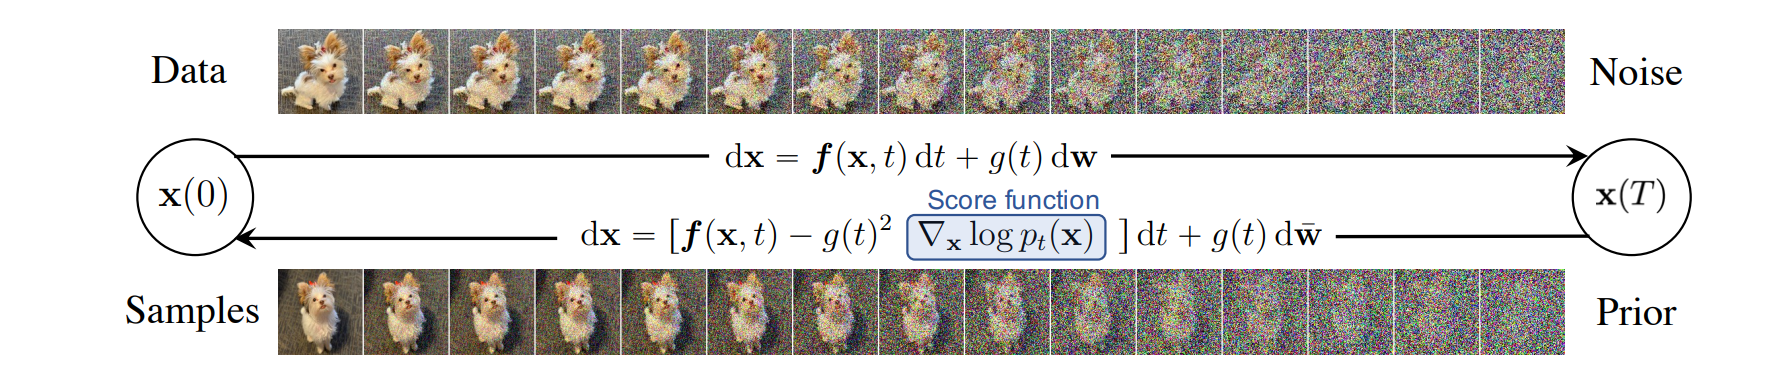
\includegraphics[width=1\linewidth]{score_based_dog.png}
    \bigskip

    We learn the score by using score-matching techniques
    \begin{block}{Score matching}
        \[\mathcal{L}_\text{score}(\theta)=\mathbb{E}\left[ \left\| s_\theta \left(\tau,\overrightarrow{X}_\tau \right)-\log p_\tau \left(\overrightarrow{X}_\tau|X_0 \right)\right\|^2  \right]   \]
    \end{block}
    Plug it in the backward process and generate by discretizing the dynamics.
\end{frame}

\begin{frame}
    Let \(X_0\sim q\) and \(f:\mathbb{R}^d\rightarrow\mathbb{R}^d\) an invertible and differentiable function an set  \(X_1:=f(X_0)\) such that \(X_1\sim p\).\\
    We can write the density of \(X_1\) as
    \begin{align}
        p_{X_1} &= p_{X_0}(f^{-1}(x_1))\left| \det \frac{\partial f^{-1}}{\partial x_1}(x_1)\right|\\
        &= p_{X_0}(f^{-1}(x_1))\left| \det \frac{\partial f}{\partial x_0}(f^{-1}(x_1))\right|^{-1} 
    \end{align}
    We can then write the log-likelihood as
    \begin{align}
        \log p_{X_1}(x_1) &= \log p_{X_0}(f^{-1}(x_1))-\log \left| \det \frac{\partial f}{\partial x_0}(f^{-1}(x_1))\right|
    \end{align}
\end{frame}

\begin{frame}{Normalizing flow}
    Let \(X_0\sim q\) and \(X_1\sim p\). We want to learn \(f_\theta\) such that \(X_1 \simeq f_\theta(X_0)=Z\sim p_Z\). To do that, we set a structure on \(f_\theta\), with \(f_1,\ldots,f_k\) simpler function (all parametrized by \(\theta\)) such that 
    \[f_\theta=f_1\circ f_2\circ\ldots\circ f_k\] 
    We determine \(f_\theta\) by minimizing 
    \[\mathcal{L}_\text{NF}(\theta)= \mathbb{E}\left[-\log p_Z(f_\theta(x))-\log \left|\det \frac{\partial f_\theta}{\partial x}(x)\right|\right]\]
\end{frame}

\begin{frame}{Flow}
    We start by defining a probability density path
    \begin{block}{Probability density path}
        A probability path \(p:[0,1]\times\mathbb{R}^d\rightarrow\mathbb{R}^d\) meaning that for each time \(t\), \(p_t\) is density function i.e. \(\int p_t(x)dx=1\).\\
    \end{block}
    A simple example of such a path is a path \(p\) interpolating two density \(p_0\) and \(p_1\) with \(p_t=tp_1+(1-t)p_0\)
    \begin{figure}[htbp]
        \centering
        \caption{A probability path interpolating $\mathcal{N}(0,0.2)$ and $\mathcal{U}([0,1])$}
    \end{figure}
\end{frame}


\begin{frame}
    \begin{figure}[h]
        \centering
        \begin{subfigure}[b]{0.8\textwidth}
          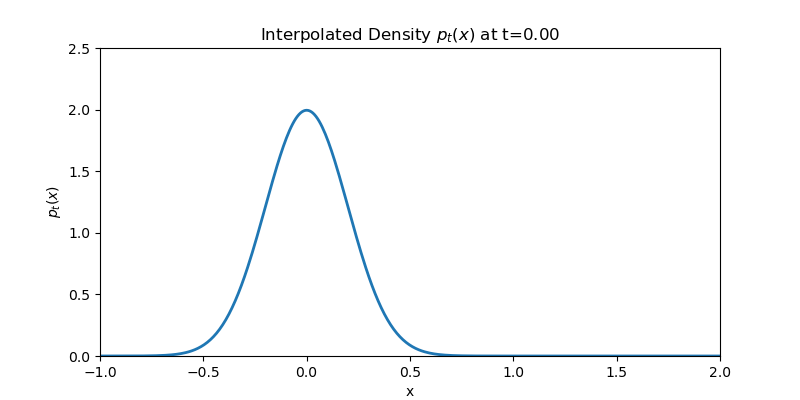
\includegraphics[width=\linewidth]{/home/admin-sbraik/Documents/InternshipProduction/FlowMatching/frames/frame_1.png}
        \end{subfigure}
        \par\medskip
        \begin{subfigure}[b]{0.8\textwidth}
          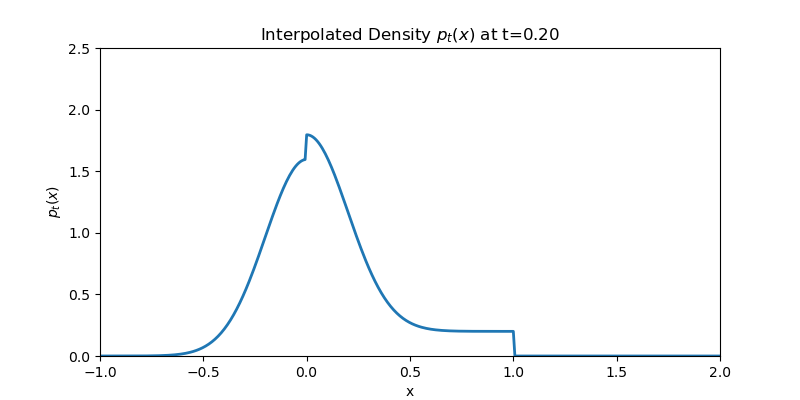
\includegraphics[width=\linewidth]{/home/admin-sbraik/Documents/InternshipProduction/FlowMatching/frames/frame_2.png}
        \end{subfigure}
    \end{figure}

\end{frame}

\begin{frame}
    \begin{figure}[htbp]
        \centering
        \begin{subfigure}[b]{0.8\textwidth}
          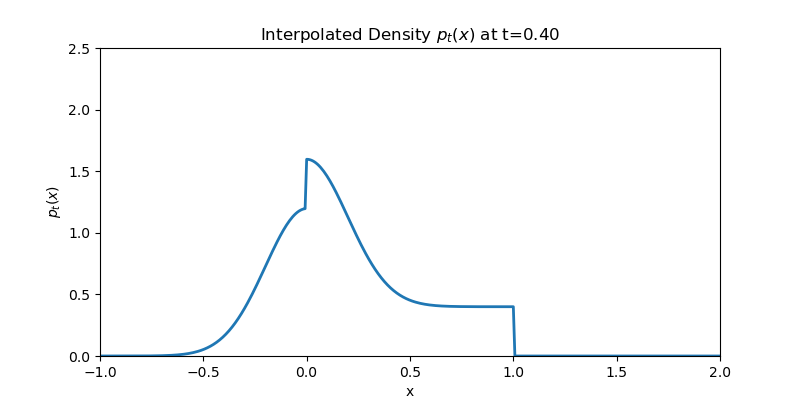
\includegraphics[width=\linewidth]{/home/admin-sbraik/Documents/InternshipProduction/FlowMatching/frames/frame_3.png}
        \end{subfigure}
        \par\medskip
        \begin{subfigure}[b]{0.8\textwidth}
          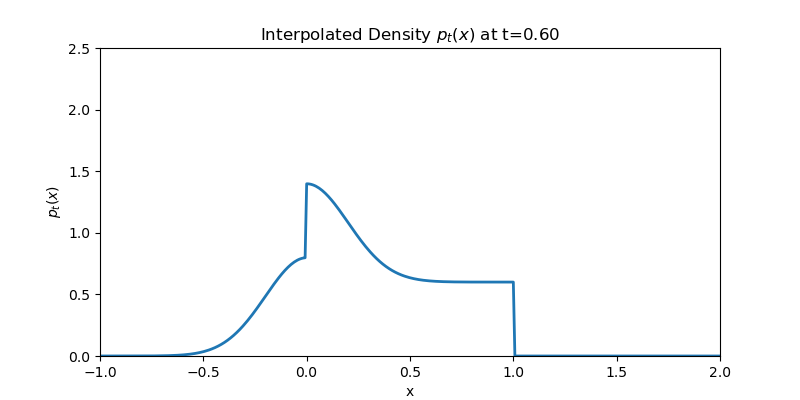
\includegraphics[width=\linewidth]{/home/admin-sbraik/Documents/InternshipProduction/FlowMatching/frames/frame_4.png}
        \end{subfigure}
    \end{figure}
\end{frame}
\begin{frame}
    \begin{figure}[htbp]
        \centering
        \begin{subfigure}[b]{0.8\textwidth}
          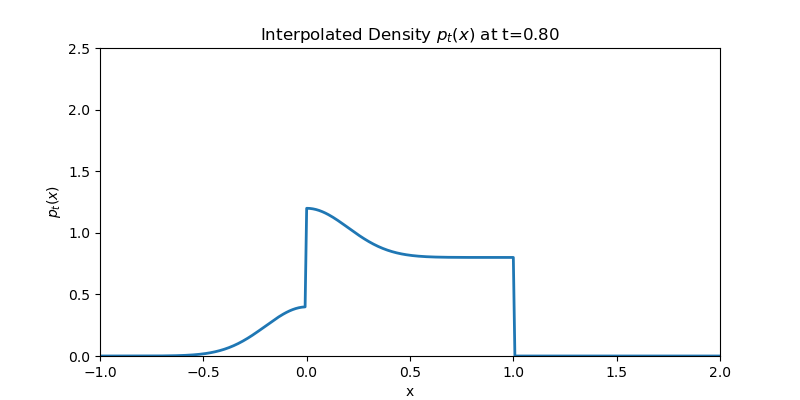
\includegraphics[width=\linewidth]{/home/admin-sbraik/Documents/InternshipProduction/FlowMatching/frames/frame_5.png}
        \end{subfigure}
        \par\medskip
        \begin{subfigure}[b]{0.8\textwidth}
          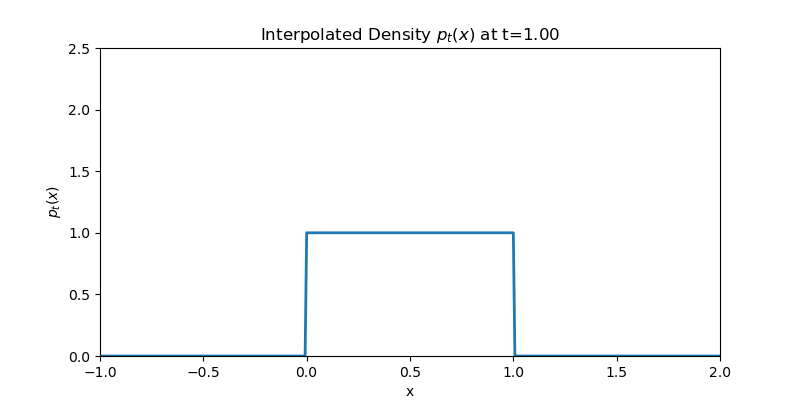
\includegraphics[width=\linewidth]{/home/admin-sbraik/Documents/InternshipProduction/FlowMatching/frames/frame_6.png}
        \end{subfigure}
        
        \label{fig:interpolated_density}
    \end{figure}
\end{frame}





\begin{frame}{Flow matching}
        The framework is as follow : \\
        We define a probability path \(p_t\) interpolating from \(p_0=q\) to \(p_1=1\). Then we learn a velocity field \(v_t^\theta\) generating the path \(p_t\) by minimizing the flow matching loss
        \begin{align}
            \mathcal{L}_\text{FM}(\theta):=\mathbb{E}[\|v_t^\theta(X_t)-\dot{X}_t \|^2]+c
        \end{align}
    Finally, we can sample from \(p_1\) by solving the ODE \eqref{ODE} with the learned velocity field \(v_t^\theta\) and the initial condition \(X_0\sim q\).
\end{frame}



\begin{frame}{Comparison}
    \begin{tabular}{|c|c|c|}
        \hline
        Models & Pros & Cons \\
        \hline
        Diffusion & 1.2 &  \\
        Normalizing flow & \makecell{Exact density estimation} & \makecell{Computationaly intensive} \\ 
        Flow matching & \makecell{Exact density estimation \\ Simulation free training}  & \makecell{test}\\
        Kernel estimator & \makecell{Flexible Easy to exploit}  & \makecell{Slow rate of convergence \\ Hard to evaluate at new data point \\ Hard to choose tuning parameters}\\
        \hline
    \end{tabular}
\end{frame}



\end{document}